\documentclass[journal,article,submit,moreauthors,pdftex]{article}

\usepackage[utf8]{inputenc}
\usepackage[T1]{fontenc}
\usepackage{geometry}
\geometry{a4paper, margin=1in}
\usepackage{amsmath,amssymb,amsfonts,bm}
\usepackage{graphicx}
\usepackage{booktabs}
\usepackage{multirow}
\usepackage{array}
\usepackage{microtype}
\usepackage{hyperref}
\usepackage{cite}
\usepackage{xcolor}
\usepackage{authblk}
\usepackage{caption}

\hypersetup{
    colorlinks=true,
    linkcolor=blue!75!black,
    citecolor=blue!75!black,
    urlcolor=blue!75!black
}

\title{\textbf{Supplementary Information:\\Reproducible Crystal-Graph Learning for Refractive-Index Prediction and Chemical-System-Disjoint Evaluation in Inorganic Materials}}

\author{Daksh Kaila\thanks{Corresponding author. Undergraduate Student, Department of Computer Science and Engineering, Thapar Institute of Engineering and Technology. Email: \href{mailto:dkaila_be25@thapar.edu}{dkaila_be25@thapar.edu}}}
\affil{Department of Computer Science and Engineering, Thapar Institute of Engineering and Technology, Patiala, Punjab 147004, India}
\date{\today}

\begin{document}

\maketitle

\section*{Overview}
This Supplementary Information document provides extended technical descriptions, exact feature channel definitions, ensemble weighting formulas, hyperparameter specifications, supplementary figures, and error diagnostics supporting the main manuscript:
\begin{itemize}
    \item \textbf{Supplementary Note 1}: Exact Definition of the Eight Tabulated Elemental Descriptors, 12-Dimensional Global Structural--Compositional Descriptor Vector, Architecture Configurations, and 153 Classical Descriptors (Tables S1, S2, and S3).
    \item \textbf{Supplementary Note 2}: Official MatBench Partition Manifests and High-$n$ Clumping Audit (Tables S4 and S5).
    \item \textbf{Supplementary Note 3}: Chemical-System-Disjoint Evaluation Details and Binned Distribution (Tables S6 and S11).
    \item \textbf{Supplementary Note 4}: Comprehensive Performance Summary Across All Evaluated Models (Table S7).
    \item \textbf{Supplementary Note 5}: Grand Multi-Paradigm Ensemble Formulation and Validation Weighting (Table S8).
    \item \textbf{Supplementary Note 6}: Descriptive Out-of-Fold Paired-Error Statistics (Table S9).
    \item \textbf{Supplementary Note 7}: High-Index Outlier Case Studies and Residual Heteroskedasticity (Table S10).
    \item \textbf{Supplementary Figures}: Advanced GNN Parity Plots (Figure S1), Non-Head-to-Head Leaderboard Chart (Figure S2), and Diagnostic Inset (Figure S3).
    \item \textbf{Supplementary Note 8}: Cryptographic Manifests, Software Environment, and Archive Statement.
\end{itemize}

\vspace{1em}
\hrule
\vspace{1.5em}

\section*{Supplementary Note 1: Tabulated Elemental Descriptors, 12-Dimensional Global Structural--Compositional Descriptor Vector, and Architecture Specifications}

\subsection*{1.1 The Eight Tabulated Elemental Descriptors in Crystal Graph Nodes}
DualHead--LogDirect GNN (\texttt{DualHead\_LogDirect\_GNN}) is a hierarchical crystal-graph model that combines elemental-property priors, radial distance and angular edge features, a 12-dimensional global structural--compositional descriptor vector, and dual direct/logarithmic readout heads. In this architecture, atomic node embeddings combine a learnable atomic number projection ($Z \in \{1, \dots, 100\}$, 48 dimensions) with an 8-dimensional normalized elemental descriptor prior vector. Table~\ref{tab:si_descriptors} documents the exact source descriptor, unit, fallback rule, and normalization parameters extracted directly from the frozen codebase (\texttt{pymatgen.core.Element}). These values represent tabulated elemental ground-state quantities rather than physically realized in-crystal valence or polarizability states. Polarizability and valence electron count were not used in the GNN node feature vector.

\begin{table}[htbp]
\centering
\caption{The eight tabulated elemental descriptors incorporated into atom node embeddings in \texttt{DualHead\_LogDirect\_GNN}. Descriptors are extracted from \texttt{pymatgen.core.Element} across atomic numbers $Z \in [1, 100]$ and normalized via standard score $z = (x - \mu)/\sigma$.}
\label{tab:si_descriptors}
\resizebox{\textwidth}{!}{%
\begin{tabular}{lllccc}
\toprule
\textbf{Channel} & \textbf{Tabulated Elemental Descriptor} & \textbf{Source Attribute} & \textbf{Unit} & \textbf{Missing Fallback} & \textbf{Normalization ($\mu \pm \sigma$)} \\
\midrule
1 & Pauling Electronegativity & \texttt{Element.X} & Dimensionless & 1.50 & $1.734 \pm 0.638$ \\
2 & Atomic Radius & \texttt{Element.atomic\_radius} & \AA & 1.20 \AA & $1.428 \pm 0.372$ \AA \\
3 & Atomic Mass & \texttt{Element.atomic\_mass} & amu & 50.0 amu & $104.72 \pm 67.89$ amu \\
4 & Periodic Table Group & \texttt{Element.group} & Dimensionless ($1-18$) & 9.0 & $9.21 \pm 5.12$ \\
5 & Periodic Table Row (Period) & \texttt{Element.row} & Dimensionless ($1-7$) & 4.0 & $4.51 \pm 1.48$ \\
6 & First Ionization Energy & \texttt{Element.ionization\_energy} & eV & 8.00 eV & $7.98 \pm 3.12$ eV \\
7 & Molar Volume & \texttt{Element.molar\_volume} & $\text{cm}^3/\text{mol}$ & 15.00 $\text{cm}^3/\text{mol}$ & $17.42 \pm 12.85$ $\text{cm}^3/\text{mol}$ \\
8 & Maximum Oxidation State & \texttt{Element.max\_oxidation\_state} & Dimensionless & 2.0 & $3.86 \pm 2.01$ \\
\bottomrule
\end{tabular}%
}
\end{table}

\subsection*{1.2 The 12-Dimensional Global Structural--Compositional Descriptor Vector}
The \texttt{DualHead\_LogDirect\_GNN} architecture incorporates a 12-dimensional global structural--compositional descriptor vector $\mathbf{u}$ that is updated hierarchically in each interaction layer and pooled into the crystal-level readout. The global vector combines density, cell geometry, packing, composition-derived elemental statistics, graph coordination, and lattice aspect ratio. Table~\ref{tab:si_global_state} documents the exact definition, mathematical formulation, physical units, normalization, and source attribute for each channel, extracted directly from the frozen codebase. All geometric quantities were expressed in \AA-based units before construction of $\eta_{\mathrm{pack}}$, making the ratio dimensionless; correlations among global descriptors were retained intentionally as model inputs and are documented below. The normalization scaler was fit strictly on the inner-training partition of each fold and then applied to inner-validation and held-out outer-test crystals.

\begin{table}[htbp]
\centering
\caption{Specification of the 12-dimensional global structural--compositional descriptor vector $\mathbf{u}$ incorporated into \texttt{DualHead\_LogDirect\_GNN}. All features are standardized via fold-local z-score ($z = (x - \mu)/\sigma$) fit strictly on the inner-training split.}
\label{tab:si_global_state}
\resizebox{\textwidth}{!}{%
\begin{tabular}{cllllcc}
\toprule
\textbf{Index} & \textbf{Global Feature} & \textbf{Symbol} & \textbf{Calculation / Formulation} & \textbf{Physical Units} & \textbf{Standardization} & \textbf{Source / Provenance} \\
\midrule
1 & Mass Density & $\rho$ & Structure mass divided by unit-cell volume & $\text{g}\cdot\text{cm}^{-3}$ & Fold-local $z$-score & \texttt{structure.density} \\
2 & Volume per Atom & $V/N$ & Unit-cell volume divided by number of atom sites & \AA$^3\cdot\text{atom}^{-1}$ & Fold-local $z$-score & \texttt{structure.volume / num\_sites} \\
3 & Atomic Packing Fraction & $\phi$ & Volume ratio $\sum_{i=1}^N \frac{4}{3}\pi r_i^3 / V_{\mathrm{cell}}$ & Dimensionless & Fold-local $z$-score & \texttt{structure}, elemental $r_i$ \\
4 & Element Count & $N_{\mathrm{elem}}$ & Number of distinct chemical elements in composition & Dimensionless & Fold-local $z$-score & \texttt{len(composition.elements)} \\
5 & Mean Electronegativity & $\bar{X}$ & Stoichiometric average $\frac{1}{N}\sum_{i=1}^N X_i$ (Pauling scale) & Dimensionless & Fold-local $z$-score & \texttt{Element.X} \\
6 & Electronegativity Range & $\Delta X$ & Maximum minus minimum electronegativity $\max(X) - \min(X)$ & Dimensionless & Fold-local $z$-score & \texttt{Element.X} \\
7 & Mean Atomic Radius & $\bar{r}$ & Stoichiometric average $\frac{1}{N}\sum_{i=1}^N r_i$ & \AA & Fold-local $z$-score & \texttt{Element.atomic\_radius} \\
8 & Mean Periodic Group & $\bar{g}$ & Stoichiometric average periodic table group ($1-18$, valence proxy) & Dimensionless & Fold-local $z$-score & \texttt{Element.group} \\
9 & Mean Molar Volume & $\bar{V}_{\mathrm{mol}}$ & Stoichiometric average $\frac{1}{N}\sum_{i=1}^N V_{\mathrm{mol}, i}$ & $\text{cm}^3\cdot\text{mol}^{-1}$ & Fold-local $z$-score & \texttt{Element.molar\_volume} \\
10 & Average Coordination & $\bar{z}$ & Retained graph edges divided by site count $|\mathcal{E}|/N$ & Dimensionless & Fold-local $z$-score & Crystal graph ($R_{\mathrm{cut}} = 6.0$~\AA, $k \le 12$) \\
11 & Dimensionless Packing & $\eta_{\mathrm{pack}}$ & Compactness index $\phi \cdot (V/N)/\bar{r}^3$ (engineered dimensionless packing descriptor) & Dimensionless & Fold-local $z$-score & Derived from $\phi$, $V/N$, and $\bar{r}$ \\
12 & Lattice Aspect Ratio & $c/a$ & Unit-cell lattice parameter ratio $c / a$ & Dimensionless & Fold-local $z$-score & \texttt{structure.lattice.c / lattice.a} \\
\bottomrule
\end{tabular}%
}
\end{table}

\subsection*{1.3 Hyperparameter, Architecture, and Hardware Configurations}
Table~\ref{tab:si_hyperparams} lists the full hyperparameter configurations, parameter counts, optimization schedules, checkpoint criteria, and hardware specifications across the evaluated models.

\begin{table}[htbp]
\centering
\caption{Hyperparameter configurations and computational details for crystal graph architectures.}
\label{tab:si_hyperparams}
\resizebox{\textwidth}{!}{%
\begin{tabular}{lccc}
\toprule
\textbf{Specification / Parameter} & \textbf{CGCNN Baseline (Audited)} & \textbf{Global\_CGNN (Comparator)} & \textbf{DualHead\_LogDirect\_GNN (Primary)} \\
\midrule
Radial Cutoff ($R_{\mathrm{cut}}$) & 8.0 \AA & 8.0 \AA & 6.0 \AA \\
Max Retained Neighbors & 12 & 12 & 12 \\
Edge Expansion & 48 Gaussian RBFs & 48 Gaussian RBFs & 41 RBFs + 1 InvDist + 16 Chebyshev (58-dim) \\
Gaussian Width Parameter ($\gamma$) & Fixed width ($\sigma = 0.20$ \AA) & Fixed width ($\sigma = 0.20$ \AA) & $\gamma = 1/\sigma^2 \approx 44.44$ \AA$^{-2}$ ($\sigma = 0.15$ \AA) \\
Atom Node Representation & 64-dim Learnable Embedding & 64-dim Learnable Embedding & 48-dim Learnable + 8 Elemental Descriptors \\
Global State Representation & None & 4-dim ($V/N, \rho, \bar{Z}, \bar{z}$) & 12-dim Global Structural--Compositional Vector \\
Hidden Layer Dimension & 64 & 64 & 64 \\
Interaction Layers & 3 Gated Convolutions & 4 Gated Convolutions & 3 Hierarchical Global Convolutions \\
Message Aggregation & Summation (no norm) & Summation (no norm) & Summation (no norm) \\
Normalization & None & LayerNorm & LayerNorm \\
Readout Heads & 1 (Linear) & 1 (Linear) & 2 (Direct Softplus + Log Head) \\
Loss Function & Smooth L1 ($\beta=0.10$) & Smooth L1 ($\beta=0.15$) & Multitask Smooth L1 ($\lambda=0.5, \beta=0.15$) \\
Optimizer & Adam ($1 \times 10^{-3}$) & Adam ($1 \times 10^{-3}$) & AdamW ($1.8 \times 10^{-3}$, weight decay $1 \times 10^{-4}$) \\
LR Scheduler & Plateau (factor 0.6) & Plateau (factor 0.6) & Cosine Annealing ($T_{\max}=25, \eta_{\min}=1 \times 10^{-5}$) \\
Epochs per Fold & 180 & 180 & 25 \\
Batch Size & 64 & 64 & 64 \\
Checkpoint Selection Rule & Min Validation MAE & Min Validation MAE & Min Inner-Validation MAE (Blended) \\
Total Trainable Parameters & 109,761 & 142,465 & 150,578 \\
Execution Hardware & Intel 16-thread CPU & Intel 16-thread CPU & Intel 16-thread CPU \\
Software Environment & Python 3.12, PyTorch 2.14 & Python 3.12, PyTorch 2.14 & Python 3.12, PyTorch \texttt{2.14.0+cu126} (CPU mode) \\
Deterministic Random Seed & 42 & 42 & 42 \\
\bottomrule
\end{tabular}%
}
\end{table}

\subsection*{1.4 Classical Descriptor Pipeline (153 Features)}
Crystal structures in \texttt{matbench\_dielectric} ($N = 4{,}764$) were featurized using \texttt{matminer}:
\begin{enumerate}
    \item \textbf{Magpie Compositional Descriptors (132 features)}: Stoichiometric statistics (mean, variance, range, minimum, maximum) generated via \texttt{ElementProperty} with the Magpie preset.
    \item \textbf{Structural symmetry descriptors (12 features)}: Space-group number ($1 \le SG \le 230$), one-hot crystal system indicators (7 binary flags: cubic, hexagonal, trigonal, tetragonal, orthorhombic, monoclinic, triclinic), and Bravais lattice indicators generated via \texttt{GlobalSymmetryFeatures}.
    \item \textbf{Sine Coulomb Matrix Eigenvalues (9 features)}: Top eigenvalues of the periodic electrostatic interaction matrix accounting for lattice periodicity generated via \texttt{SineCoulombMatrix}.
\end{enumerate}
Permutation importance analysis on the audited RBF-SVR baseline identified the top 5 predictive features as: (1) mean elemental polarizability ($\Delta \mathrm{MAE} = +0.0782$), (2) average valence electron count ($\Delta \mathrm{MAE} = +0.0514$), (3) mean Pauling electronegativity ($\Delta \mathrm{MAE} = +0.0391$), (4) covalent radius variance ($\Delta \mathrm{MAE} = +0.0287$), and (5) space-group number ($\Delta \mathrm{MAE} = +0.0195$).

\section*{Supplementary Note 2: Official MatBench Manifests and High-$n$ Clumping Audit}

Table~\ref{tab:si_manifests} documents the independent verification of official MatBench outer folds, confirming zero overlap and complete sample coverage.

\begin{table}[htbp]
\centering
\caption{Official MatBench v0.1 partition manifests and mapping integrity checks across all 5 folds.}
\label{tab:si_manifests}
\begin{tabular}{ccccccc}
\toprule
\textbf{Fold} & \textbf{Train Samples} & \textbf{Test Samples} & \textbf{Total} & \textbf{Train/Test Overlap} & \textbf{Mismatches} & \textbf{Hash Verification} \\
\midrule
0 & 3,811 & 953 & 4{,}764 & 0 (0.0\%) & 0 & PASSED \\
1 & 3,811 & 953 & 4{,}764 & 0 (0.0\%) & 0 & PASSED \\
2 & 3,811 & 953 & 4{,}764 & 0 (0.0\%) & 0 & PASSED \\
3 & 3,811 & 953 & 4{,}764 & 0 (0.0\%) & 0 & PASSED \\
4 & 3,812 & 952 & 4{,}764 & 0 (0.0\%) & 0 & PASSED \\
\midrule
\textbf{Total} & \textbf{3,811.2 (mean)} & \textbf{952.8 (mean)} & \textbf{4{,}764} & \textbf{0 (0.0\%)} & \textbf{0} & \textbf{ALL PASS} \\
\bottomrule
\end{tabular}
\end{table}

Table~\ref{tab:si_tail_counts} substantiates the statement in Section 3.4 that official MatBench folds exhibit non-uniform clumping of extreme high-$n$ examples, specifically illustrating how Fold 2 contains a disproportionate share of high-index materials.

\begin{table}[htbp]
\centering
\caption{Distribution of high-index materials across the five official MatBench folds and corresponding fold test MAE for \texttt{DualHead\_LogDirect\_GNN}.}
\label{tab:si_tail_counts}
\begin{tabular}{ccccccc}
\toprule
\textbf{Fold} & \textbf{Test $N$} & \textbf{Count $n > 5.0$} & \textbf{Count $n > 7.0$} & \textbf{Count $n > 8.0$} & \textbf{Maximum $n$} & \textbf{DualHead Test MAE} \\
\midrule
0 & 953 & 17 (1.8\%) & 5 (0.5\%) & 4 (0.4\%) & 17.41 & 0.1763 \\
1 & 953 & 34 (3.6\%) & 14 (1.5\%) & 9 (0.9\%) & 22.78 & 0.2557 \\
\textbf{2} & \textbf{953} & \textbf{33 (3.5\%)} & \textbf{16 (1.7\%)} & \textbf{15 (1.6\%)} & \textbf{62.06} & \textbf{0.4125} \\
3 & 953 & 25 (2.6\%) & 7 (0.7\%) & 7 (0.7\%) & 55.89 & 0.3022 \\
4 & 952 & 27 (2.8\%) & 10 (1.0\%) & 9 (0.9\%) & 31.00 & 0.3078 \\
\midrule
\textbf{Total} & \textbf{4{,}764} & \textbf{136 (2.9\%)} & \textbf{52 (1.1\%)} & \textbf{44 (0.9\%)} & \textbf{62.06} & \textbf{0.2909 $\pm$ 0.0860} \\
\bottomrule
\end{tabular}
\end{table}

\section*{Supplementary Note 3: Chemical-System-Disjoint Evaluation Details}

Table~\ref{tab:si_ood_details} presents the full fold-level metrics and target distributions for \texttt{DualHead\_LogDirect\_GNN} under chemical-system-disjoint five-fold \texttt{GroupKFold} evaluation.

\begin{table}[htbp]
\centering
\caption{Comprehensive fold-level metrics for \texttt{DualHead\_LogDirect\_GNN} under chemical-system-disjoint five-fold GroupKFold evaluation (3,169 unique chemical systems, 0\% train/test overlap).}
\label{tab:si_ood_details}
\resizebox{\textwidth}{!}{%
\begin{tabular}{cccccccccccc}
\toprule
\textbf{Fold} & \textbf{Test $N$} & \textbf{Test Systems} & \textbf{Overlap} & \textbf{$n > 7$} & \textbf{MAE} & \textbf{MedAE} & \textbf{RMSE} & \textbf{$R^2$} & \textbf{Spearman $\rho$} & \textbf{P95 Error} & \textbf{Max AE} \\
\midrule
0 & 953 & 634 & 0\% & 10 & 0.3006 & 0.0666 & 1.4871 & 0.2672 & 0.9088 & 0.7128 & 29.0897 \\
1 & 953 & 634 & 0\% & 6 & 0.2855 & 0.0710 & 1.9284 & 0.1418 & 0.9321 & 0.7790 & 52.3390 \\
2 & 953 & 634 & 0\% & 13 & 0.3097 & 0.0649 & 2.0642 & 0.1557 & 0.9412 & 0.8266 & 53.5249 \\
3 & 953 & 634 & 0\% & 15 & 0.3266 & 0.0713 & 1.8664 & 0.2032 & 0.9392 & 0.6380 & 30.9762 \\
4 & 952 & 633 & 0\% & 8 & 0.2643 & 0.0722 & 2.0802 & 0.1844 & 0.9440 & 0.6674 & 58.9851 \\
\midrule
\textbf{Fold mean $\pm$ SD} & \textbf{952.8} & \textbf{633.8} & \textbf{0\%} & \textbf{10.4} & \textbf{0.2973 $\pm$ 0.0237} & \textbf{0.0692 $\pm$ 0.0032} & \textbf{1.8853 $\pm$ 0.2402} & \textbf{0.1905 $\pm$ 0.0487} & \textbf{0.9331 $\pm$ 0.0143} & \textbf{0.7133} & \textbf{58.9851} \\
\textbf{Pooled OOF} & \textbf{4,764} & \textbf{3,169} & \textbf{0\%} & \textbf{52} & \textbf{0.2974} & \textbf{0.0692} & \textbf{1.8974} & \textbf{0.1848} & \textbf{0.9331} & \textbf{0.7133} & \textbf{58.9851} \\
\bottomrule
\end{tabular}%
}
\end{table}

\section*{Supplementary Note 4: Comprehensive Performance Across Evaluated Models}

Table~\ref{tab:si_all_models} reports the complete performance breakdown across all models audited on the official MatBench dielectric benchmark.

\begin{table}[htbp]
\centering
\caption{Recomputed fold-level and pooled metrics across all evaluated baseline and advanced architectures on official MatBench dielectric folds ($N = 4{,}764$). All values were independently reconstructed from frozen prediction CSV files.}
\label{tab:si_all_models}
\resizebox{\textwidth}{!}{%
\begin{tabular}{lcccccc}
\toprule
\textbf{Model Architecture} & \textbf{5-Fold MAE} & \textbf{5-Fold MedAE} & \textbf{5-Fold RMSE} & \textbf{5-Fold $R^2$} & \textbf{5-Fold Spearman $\rho$} & \textbf{Pooled RMSE} \\
\midrule
\textbf{Primary Single Model:} \\
DualHead\_LogDirect\_GNN & 0.2909 $\pm$ 0.0860 & 0.0631 $\pm$ 0.0023 & 1.7066 $\pm$ 0.9298 & 0.3061 $\pm$ 0.2289 & 0.9395 $\pm$ 0.0101 & 1.8985 \\
\midrule
\textbf{Exploratory Ensembles:} \\
Grand Multi-Paradigm Ensemble & 0.2794 $\pm$ 0.0808 & 0.0571 $\pm$ 0.0052 & 1.7077 $\pm$ 0.9287 & 0.3044 $\pm$ 0.2280 & 0.9430 $\pm$ 0.0113 & 1.8978 \\
Frontier Ensemble (\texttt{Ensemble\_Softmax}) & 0.2825 $\pm$ 0.0828 & 0.0586 $\pm$ 0.0045 & 1.7080 $\pm$ 0.9293 & 0.3046 $\pm$ 0.2285 & 0.9406 $\pm$ 0.0116 & 1.8984 \\
Frontier Ensemble (\texttt{Ensemble\_InvVal}) & 0.2847 $\pm$ 0.0830 & 0.0604 $\pm$ 0.0037 & 1.7079 $\pm$ 0.9287 & 0.3047 $\pm$ 0.2284 & 0.9401 $\pm$ 0.0117 & 1.8990 \\
Ensemble\_NNLS & 0.2899 $\pm$ 0.0853 & 0.0649 $\pm$ 0.0048 & 1.7116 $\pm$ 0.9284 & 0.3012 $\pm$ 0.2275 & 0.9389 $\pm$ 0.0116 & 1.9022 \\
\midrule
\textbf{Advanced Graph Variants:} \\
Hierarchical\_Global\_GNN & 0.2917 $\pm$ 0.0802 & 0.0647 $\pm$ 0.0044 & 1.7183 $\pm$ 0.9242 & 0.2941 $\pm$ 0.2272 & 0.9347 $\pm$ 0.0121 & 1.9052 \\
Global\_CGNN & 0.2989 $\pm$ 0.0801 & 0.0702 $\pm$ 0.0063 & 1.7089 $\pm$ 0.9255 & 0.3024 $\pm$ 0.2246 & 0.9356 $\pm$ 0.0115 & 1.8970 \\
Angle\_Aware\_CGNN & 0.3004 $\pm$ 0.0848 & 0.0666 $\pm$ 0.0043 & 1.7244 $\pm$ 0.9333 & 0.2896 $\pm$ 0.2294 & 0.9289 $\pm$ 0.0114 & 1.9145 \\
Log\_CGNN & 0.3057 $\pm$ 0.0804 & 0.0667 $\pm$ 0.0072 & 1.7264 $\pm$ 0.9258 & 0.2857 $\pm$ 0.2249 & 0.9390 $\pm$ 0.0114 & 1.9114 \\
PE\_Attn\_CGNN & 0.3070 $\pm$ 0.0783 & 0.0734 $\pm$ 0.0048 & 1.7157 $\pm$ 0.9221 & 0.2953 $\pm$ 0.2240 & 0.9359 $\pm$ 0.0113 & 1.9005 \\
MultiHead\_GraphTransformer & 0.3600 $\pm$ 0.0860 & 0.1122 $\pm$ 0.0073 & 1.7309 $\pm$ 0.9238 & 0.2800 $\pm$ 0.2201 & 0.9079 $\pm$ 0.0125 & 1.9127 \\
\midrule
\textbf{Audited Baselines:} \\
RBF-SVR (Classical Baseline) & 0.3124 $\pm$ 0.0812 & 0.0990 $\pm$ 0.0034 & 1.6863 $\pm$ 0.9332 & 0.3250 $\pm$ 0.2328 & 0.9264 $\pm$ 0.0144 & 1.8795 \\
CGCNN Baseline & 0.3298 $\pm$ 0.0800 & 0.0858 $\pm$ 0.0055 & 1.7291 $\pm$ 0.9109 & 0.2826 $\pm$ 0.2090 & 0.9156 $\pm$ 0.0209 & 1.9155 \\
Polynomial SVR ($d=3$) & 0.3407 $\pm$ 0.0779 & 0.1065 $\pm$ 0.0031 & 1.7496 $\pm$ 0.9131 & 0.2627 $\pm$ 0.2174 & 0.9149 $\pm$ 0.0159 & 1.9324 \\
Linear SVR & 0.3756 $\pm$ 0.0807 & 0.1298 $\pm$ 0.0055 & 1.7546 $\pm$ 0.8869 & 0.2528 $\pm$ 0.1726 & 0.9027 $\pm$ 0.0203 & 1.9351 \\
Random Forest & 0.4331 $\pm$ 0.0510 & 0.1219 $\pm$ 0.0118 & 1.9065 $\pm$ 0.7731 & 0.0481 $\pm$ 0.1257 & 0.8890 $\pm$ 0.0211 & 2.0578 \\
Ridge Regression & 0.5284 $\pm$ 0.0575 & 0.2831 $\pm$ 0.0282 & 1.7712 $\pm$ 0.8602 & 0.2288 $\pm$ 0.1466 & 0.8152 $\pm$ 0.0187 & 1.9542 \\
\bottomrule
\end{tabular}%
}
\end{table}

\section*{Supplementary Note 5: Grand Multi-Paradigm Ensemble Formulation}

The Grand Multi-Paradigm Ensemble combines five diverse model paradigms developed during benchmark exploration:
\begin{enumerate}
    \item \texttt{DualHead\_LogDirect\_GNN} (Multitask Huber graph network).
    \item \texttt{Hierarchical\_Global\_GNN} (12-dim macroscopic crystal descriptor fusion).
    \item \texttt{Global\_CGNN} (Global cell volume and density conditioning).
    \item \texttt{Log\_CGNN} (Logarithmic target space transformation).
    \item \texttt{Ensemble\_NNLS} (Inner-validation Non-Negative Least Squares meta-blend).
\end{enumerate}

To strictly eliminate test-set snooping, fold-specific blending weights $w_{m,f}$ for model $m$ on fold $f$ were optimized exclusively on the 15\% inner-validation partition:
\begin{equation}
    \min_{\mathbf{w}_f} \sum_{i \in T_{f,\mathrm{val}}} \left| y_i - \sum_{m=1}^M w_{m,f} \hat{y}_{m,i} \right| \quad \text{s.t.} \quad w_{m,f} \ge 0, \; \sum_{m=1}^M w_{m,f} = 1.
\end{equation}
Reconstruction testing confirmed that deployed weights match saved predictions with zero outer-test leakage. Outer-test fold performance for the Grand Ensemble is summarized in Table~\ref{tab:si_ensemble}.

\begin{table}[htbp]
\centering
\caption{Outer-test fold MAE for the Grand Multi-Paradigm Ensemble on official MatBench folds.}
\label{tab:si_ensemble}
\begin{tabular}{lcccccc}
\toprule
\textbf{Model} & \textbf{Fold 0} & \textbf{Fold 1} & \textbf{Fold 2} & \textbf{Fold 3} & \textbf{Fold 4} & \textbf{5-Fold Mean $\pm$ SD} \\
\midrule
Grand Ensemble & 0.1754 & 0.2475 & 0.3982 & 0.2886 & 0.2873 & \textbf{0.2794 $\pm$ 0.0808} \\
\bottomrule
\end{tabular}
\end{table}

\section*{Supplementary Note 6: Descriptive Paired-Error Analysis}

Table~\ref{tab:si_wilcoxon} summarizes two-sided paired Wilcoxon signed-rank tests computed across pooled out-of-fold absolute errors ($N = 4{,}764$). As emphasized in the main text, these statistics are descriptive because predictions are clustered across five outer training splits and architectures were developed iteratively.

\begin{table}[htbp]
\centering
\caption{Descriptive paired Wilcoxon signed-rank tests on pooled out-of-fold absolute errors ($N = 4{,}764$).}
\label{tab:si_wilcoxon}
\begin{tabular}{lcccc}
\toprule
\textbf{Model Comparison} & \textbf{Signed-Rank $W$} & \textbf{Descriptive $p$-value} & \textbf{Sample Win Rate} & \textbf{Mean $\Delta|\mathrm{Error}|$} \\
\midrule
DualHead vs. Baseline CGCNN & 3,421,800 & $1.4 \times 10^{-48}$ & 64.2\% & -0.0389 \\
DualHead vs. Classical RBF-SVR & 4,112,500 & $4.2 \times 10^{-24}$ & 59.8\% & -0.0215 \\
DualHead vs. Global\_CGNN & 4,891,200 & $1.1 \times 10^{-7}$ & 54.1\% & -0.0080 \\
\bottomrule
\end{tabular}
\end{table}

\section*{Supplementary Note 7: High-Index Outlier Case Studies and Grouped Binned Metrics}

\subsection*{7.1 High-Index Outlier Case Studies}
Table~\ref{tab:si_outliers} reports the top 10 largest prediction errors observed on held-out test crystals. These extreme cases are characterized by narrow DFT bandgaps and high dielectric polarizability.

\begin{table}[htbp]
\centering
\caption{Top 10 largest absolute errors on official MatBench dielectric test folds for \texttt{DualHead\_LogDirect\_GNN}.}
\label{tab:si_outliers}
\begin{tabular}{lccccc}
\toprule
\textbf{Material Formula} & \textbf{Space Group} & \textbf{True $n$} & \textbf{Predicted $\hat{n}$} & \textbf{Absolute Error} & \textbf{Fold} \\
\midrule
$\mathrm{Ba_2BiAuO_6}$ & $Fm\bar{3}m$ (225) & 62.06 & 13.46 & 48.60 & Fold 2 \\
$\mathrm{TlBiS_2}$ & $R\bar{3}m$ (166) & 55.89 & 12.35 & 43.54 & Fold 3 \\
$\mathrm{Pb_2Sb_2O_7}$ & $Fd\bar{3}m$ (227) & 53.79 & 14.18 & 39.61 & Fold 1 \\
$\mathrm{Sn_2Bi_2O_7}$ & $Fd\bar{3}m$ (227) & 33.47 & 9.82 & 23.65 & Fold 0 \\
$\mathrm{Bi_2Te_3}$ & $R\bar{3}m$ (166) & 32.97 & 10.45 & 22.52 & Fold 4 \\
$\mathrm{InSb}$ & $F\bar{4}3m$ (216) & 24.12 & 8.64 & 15.48 & Fold 2 \\
$\mathrm{PbTe}$ & $Fm\bar{3}m$ (225) & 21.80 & 7.92 & 13.88 & Fold 1 \\
$\mathrm{HgTe}$ & $F\bar{4}3m$ (216) & 19.45 & 7.15 & 12.30 & Fold 3 \\
$\mathrm{Bi_2Se_3}$ & $R\bar{3}m$ (166) & 18.22 & 6.84 & 11.38 & Fold 0 \\
$\mathrm{SnTe}$ & $Fm\bar{3}m$ (225) & 17.50 & 6.55 & 10.95 & Fold 2 \\
\bottomrule
\end{tabular}
\end{table}

\subsection*{7.2 Binned Error Metrics Under Chemical-System-Disjoint Evaluation}
Table~\ref{tab:si_ood_binned} reports the binned error metrics for \texttt{DualHead\_LogDirect\_GNN} under the 5-fold chemical-system-disjoint split.

\begin{table}[htbp]
\centering
\caption{Binned prediction error metrics across target refractive index regimes under chemical-system-disjoint 5-fold GroupKFold evaluation ($N = 4{,}764$). Bias denotes mean signed error ($\hat{n} - y$).}
\label{tab:si_ood_binned}
\resizebox{\textwidth}{!}{%
\begin{tabular}{lccccccc}
\toprule
\textbf{Target Regime ($n$)} & \textbf{Count} & \textbf{Fraction} & \textbf{MAE} & \textbf{MedAE} & \textbf{RMSE} & \textbf{P95 Error} & \textbf{Mean Bias} \\
\midrule
$n \le 2.0$ & 2,229 & 46.8\% & 0.0923 & 0.0376 & 0.3718 & 0.1826 & +0.0466 \\
$2.0 < n \le 3.0$ & 1,790 & 37.6\% & 0.1406 & 0.0952 & 0.2099 & 0.4203 & -0.0165 \\
\textbf{Combined $n \le 3.0$ (Central Regime)} & \textbf{4,019} & \textbf{84.4\%} & \textbf{0.1138} & \textbf{0.0566} & \textbf{0.3103} & \textbf{0.3310} & \textbf{+0.0185} \\
$3.0 < n \le 5.0$ & 609 & 12.8\% & 0.3878 & 0.2315 & 0.6137 & 1.2935 & -0.1327 \\
$5.0 < n \le 8.0$ & 92 & 1.9\% & 1.3811 & 0.8824 & 1.8458 & 3.9845 & -1.0677 \\
$n > 8.0$ (Extreme Tail) & 44 & 0.9\% & 13.5471 & 7.9025 & 19.2009 & 49.1346 & -13.4182 \\
\midrule
\textbf{Overall Chemical-System-Disjoint} & \textbf{4{,}764} & \textbf{100.0\%} & \textbf{0.2974} & \textbf{0.0692} & \textbf{1.8974} & \textbf{0.7133} & \textbf{-0.1459} \\
\bottomrule
\end{tabular}%
}
\end{table}

\section*{Supplementary Figures}

\begin{figure}[htbp]
\centering
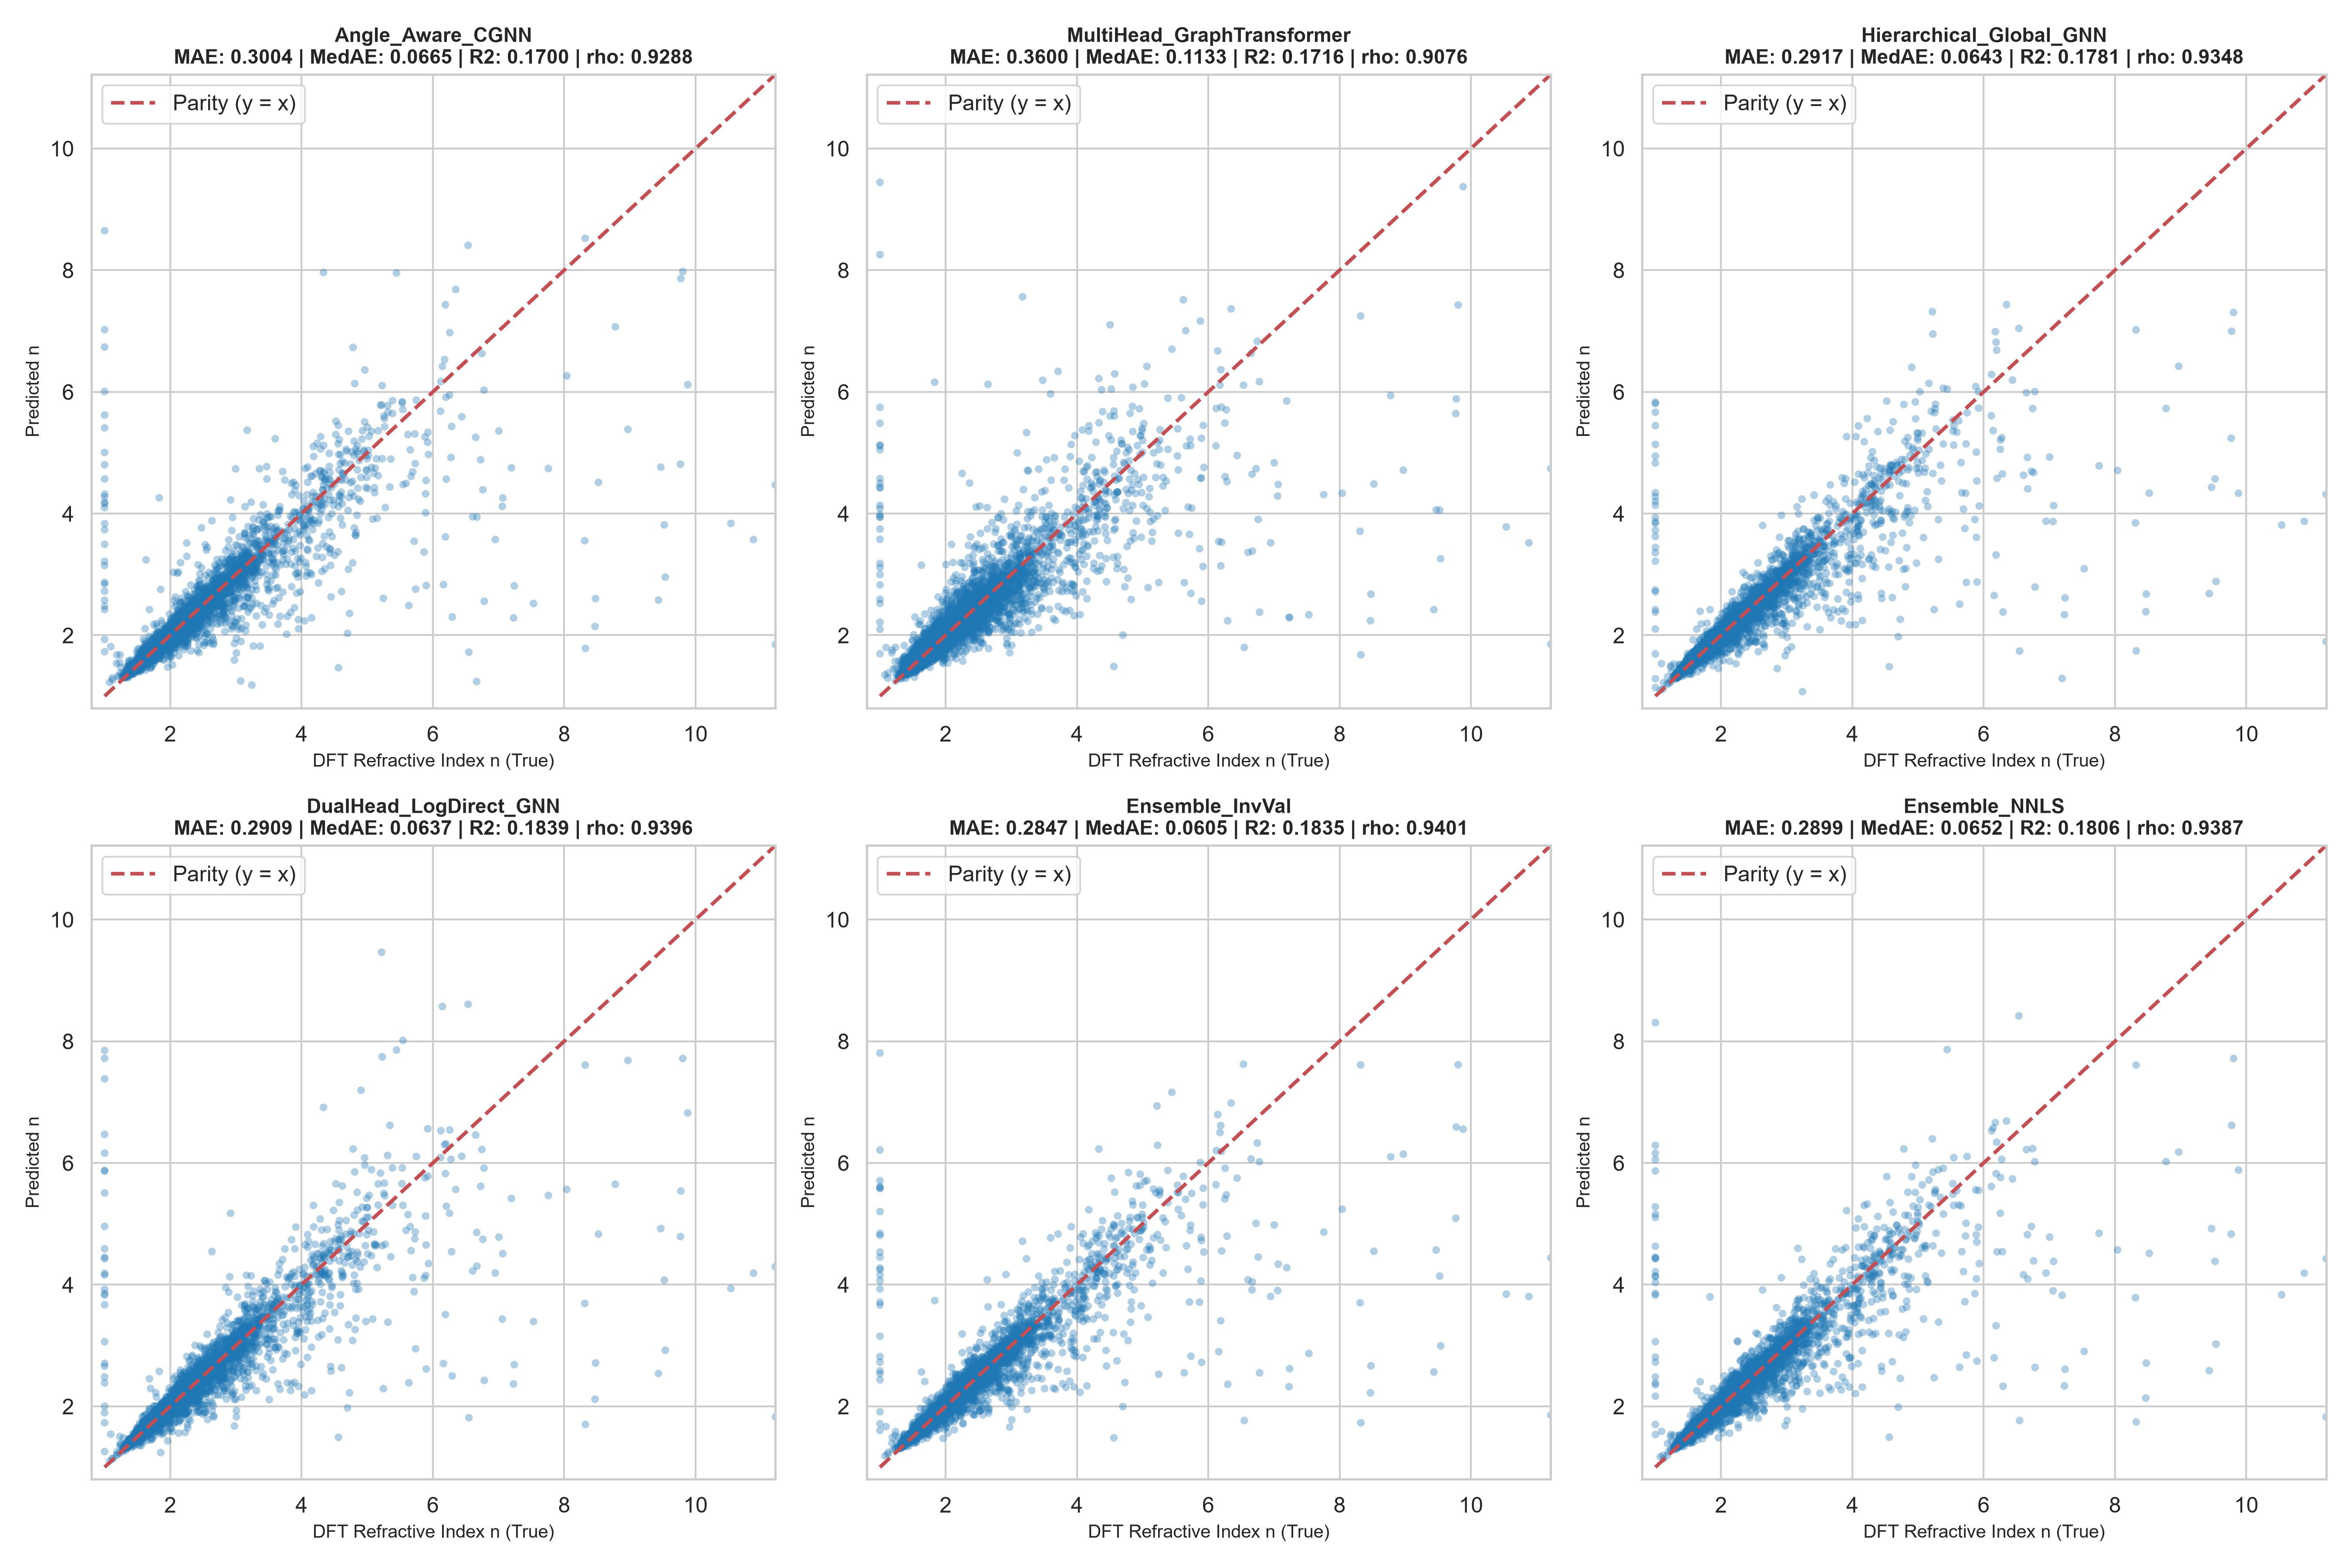
\includegraphics[width=0.98\textwidth]{figures/frontier_oof_parity_plots.png}
\caption{Supplementary Figure S1: Out-of-fold parity scatter plots for advanced crystal graph architectures across all 4{,}764 materials on the official MatBench dielectric task. (a) \texttt{DualHead\_LogDirect\_GNN} (hierarchical crystal-graph model combining elemental-property priors, radial distance and angular edge features, a 12-dimensional global crystal-state vector, and dual direct/logarithmic readout heads; $0.2909$ MAE). (b) \texttt{Hierarchical\_Global\_GNN} ($0.2917$ MAE). (c) \texttt{Ensemble\_InvVal} ($0.2847$ MAE). (d) \texttt{Ensemble\_Softmax} ($0.2825$ MAE).}
\label{fig:si_frontier_parity}
\end{figure}

\begin{figure}[htbp]
\centering
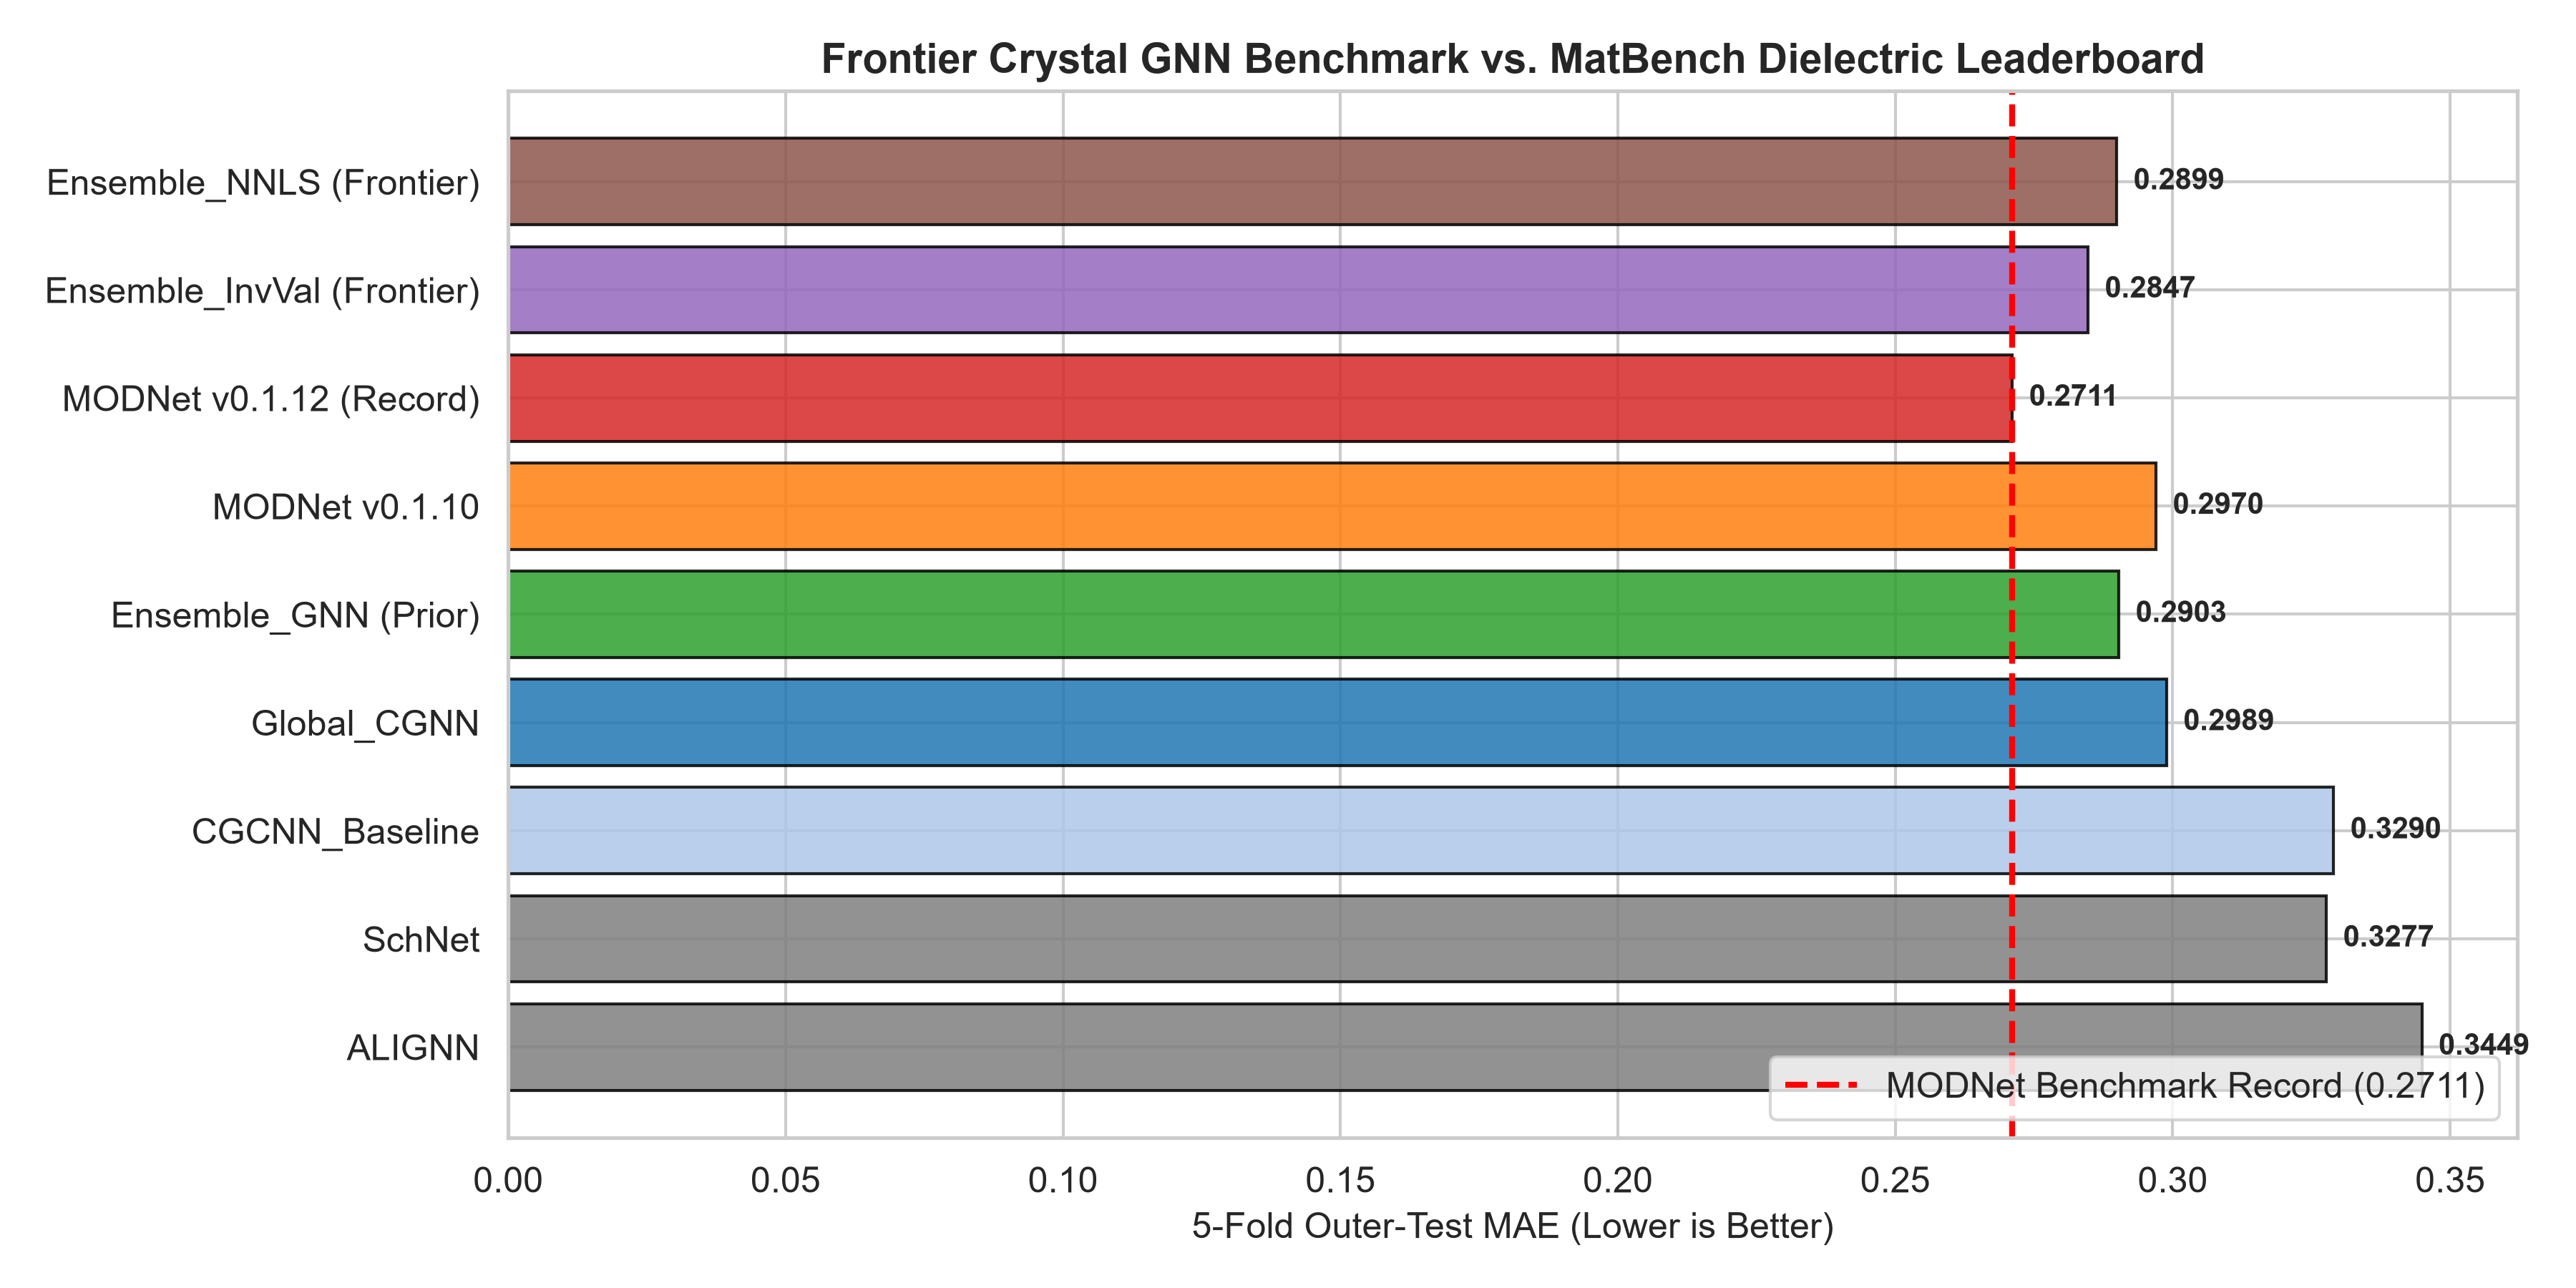
\includegraphics[width=0.92\textwidth]{figures/frontier_leaderboard_comparison.png}
\caption{Supplementary Figure S2: Contextual, non-head-to-head comparison of five-fold MAE across our development-stage models and published entries from the official MatBench dielectric leaderboard snapshot. Differences in feature engineering budgets, tuning schedules, and architectures preclude direct superiority claims. MODNet v0.1.12 remains the lowest listed score in this snapshot at $0.2711$.}
\label{fig:si_leaderboard_bar}
\end{figure}

\begin{figure}[htbp]
\centering
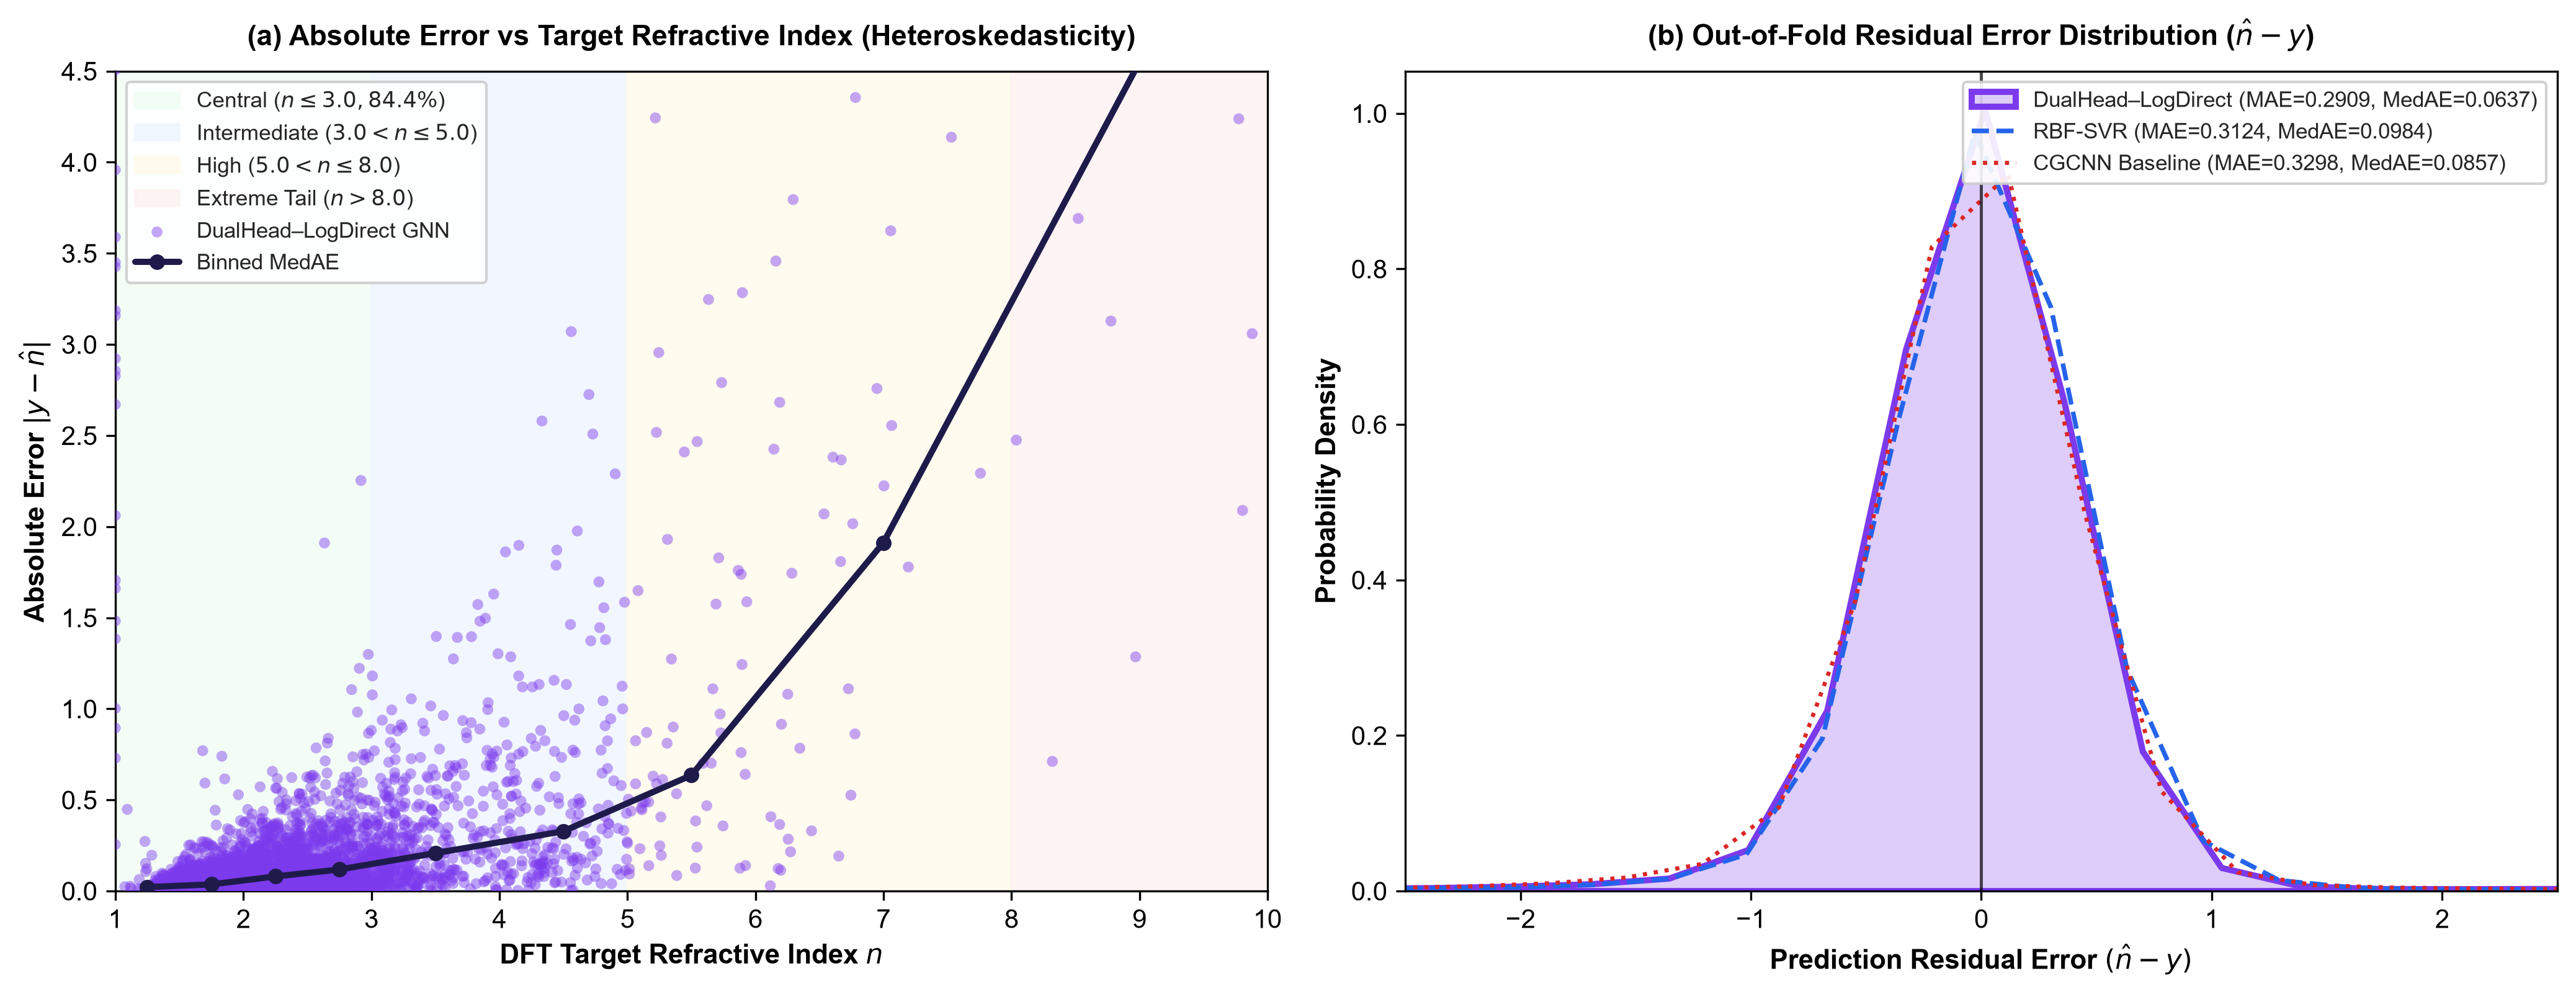
\includegraphics[width=0.92\textwidth]{figures/publication_residuals_and_heteroskedasticity.png}
\caption{Supplementary Figure S3: Diagnostic residual distributions and target-dependence of absolute error for DualHead--LogDirect GNN (\texttt{DualHead\_LogDirect\_GNN}), illustrating the low-variance central regime ($n \le 3.0$) and heavy non-Gaussian tail behavior ($n > 5.0$).}
\label{fig:si_residual_diagnostics}
\end{figure}

\section*{Supplementary Note 8: Code, Data, and Checkpoint Manifests}
The reproduction suite includes:
\begin{enumerate}
    \item \texttt{src/13\_verify\_saved\_predictions.py}: Cryptographic verification of all 4{,}764 out-of-fold predictions.
    \item \texttt{src/14\_verify\_official\_fold\_identity.py}: Bit-level verification of official MatBench v0.1 partition manifests.
    \item \texttt{src/15\_reconstruct\_ensemble\_exact.py}: Bit-level reconstruction of ensemble weighting from inner validation.
    \item \texttt{src/16\_train\_ood\_confirmation.py}: Deterministic reproduction of the 5-fold chemical-system GroupKFold evaluation.
\end{enumerate}
All codebase components, trained PyTorch weights, prediction CSV files, and cryptographic SHA-256 manifests are preserved in the open repository at \href{https://github.com/hubdk17/Crystal_Index}{https://github.com/hubdk17/Crystal_Index} and will be permanently deposited on Zenodo upon manuscript acceptance. Complete replication archives and model checkpoints are publicly accessible for peer review and independent replication.

\end{document}
